%%%%%%%%%%%%%%
% THINGS TO DO NOW %
%%%%%%%%%%%%%%


% Stickman drawing
% Actually replot the schelling stuff properly.


\documentclass[12pt]{beamer}
\setbeamerfont{frametitle}{size=\large, series=\bfseries}
\setbeamertemplate{frametitle}{%
    \vskip-10pt% Adjust this value to move the frametitle closer to the top
    \insertframetitle%
    \vskip-5pt% Adjust this value to change the space below the frametitle
}
\setbeamertemplate{navigation symbols}{}%remove navigation symbols

\usepackage{minted}
\usepackage{booktabs}
\usepackage{multicol}
\usepackage{tabularx}
\usepackage{makecell}
\usepackage{transparent}
\usepackage{soul}
\usepackage{ulem}
\usepackage{wasysym}
\usepackage{hyperref}
\usepackage{subcaption}
\usepackage{listings}
\usepackage{fancyvrb}
\usepackage{multicol}
\usepackage{booktabs}
\usepackage[document]{ragged2e}
\usepackage[english]{babel}
\usepackage{blindtext}
\usepackage{ragged2e}
\usepackage{adjustbox}
\usepackage{amsmath}
\usepackage{tcolorbox}
\usepackage{graphicx}
\usepackage{animate}
\renewcommand{\ULthickness}{1pt}
\captionsetup{justification=raggedright,singlelinecheck=false}

\newenvironment{myenv}[1]
  {\mdfsetup{
    frametitle={\colorbox{white}{\space#1\space}},
    innertopmargin=0pt,
    frametitleaboveskip=-\ht\strutbox,
    frametitlealignment=\center,
    linewidth=1pt,
    roundcorner=10pt
    }
  \begin{mdframed}%
  }
  {\end{mdframed}}

\useoutertheme{infolines}
\usepackage{newpxtext,newpxmath}
%\usepackage{mathpazo}

\usepackage[framemethod=tikz]{mdframed}
\usetikzlibrary{shadows}
\usepackage{pdfpages}
\newmdenv[shadow=true,shadowcolor=black,font=\sffamily,rightmargin=8pt]{shadedbox}
\usepackage{pifont,xcolor}
\definecolor{myblue}{RGB}{49,54,149}
\definecolor{myred}{RGB}{165,0,38}

\definecolor{myorange}{RGB}{255,120,0}
\definecolor{mygreen}{RGB}{76, 187, 23}

\definecolor{grayedout}{RGB}{225,225,225}
\usepackage{graphicx}
\usepackage{caption}
\usepackage{amsmath}
\newcommand{\icol}[1]{% inline column vector
  \left(\begin{smallmatrix}#1\end{smallmatrix}\right)%
}
\newcommand{\lenitem}[2][.55\linewidth]{figures//\parbox[t]{#1}{#2\strut \strut \justify \justifying}}

\usetheme{Frankfurt}

%   \usefonttheme{professionalfonts}
\newenvironment{variableblock}[3]{%
  \setbeamercolor{block body}{#2}
  \setbeamercolor{block title}{#3}
  \begin{block}{#1}}{\end{block}}
\usecolortheme{dove}
%\usecolortheme{rose}
%\usecolortheme{whale}

\usefonttheme[onlymath]{serif}  % only math serif font
\usefonttheme{serif}

\setbeamercolor{block title}{bg=white,fg=black}
\newcommand{\itemcolor}[1]{% Update list item colour
  \renewcommand{\makelabel}[1]{\color{#1}\hfil ##1}}

\newcounter{tmpc}
\setbeamercolor{section in head/foot}{fg=black, bg=white}
\setbeamercolor{enumerate item}{ fg=myred}
\setbeamertemplate{frametitle}
{
    \nointerlineskip
    \begin{beamercolorbox}[sep=0.3cm,ht=1.8em,wd=\paperwidth]{frametitle}
        \vbox{}\vskip-3ex%
        \strut\insertframetitle\strut
        \vskip-1.2ex%
    \end{beamercolorbox}
}
\addtobeamertemplate{frametitle}{\vskip0.5ex}{}
\makeatletter
\setbeamertemplate{footline}
{
  \leavevmode%
  \hbox{%
  \begin{beamercolorbox}[wd=.875 \paperwidth,ht=2.25ex,dp=1ex,left]{section in head/foot}%
    \usebeamerfont{author in head/foot}\quad \quad \insertshorttitle
 \end{beamercolorbox}%
 \begin{beamercolorbox}[wd=.125\paperwidth,ht=2.25ex,dp=1ex,right]{section in head/foot}%
    \usebeamerfont{date in head/foot} \quad \quad
    \insertframenumber{} / \inserttotalframenumber\hspace*{2ex}
  \end{beamercolorbox}}%
  \vskip0pt%
}
\let\@@magyar@captionfix\relax



\newcommand\jsonkey{\color{purple}}
\newcommand\jsonvalue{\color{cyan}}
\newcommand\jsonnumber{\color{orange}}

% switch used as state variable
\makeatletter
\newif\ifisvalue@json

\lstdefinelanguage{json}{
    tabsize             = 4,
    showstringspaces    = false,
    keywords            = {false,true},
    alsoletter          = 0123456789.,
    morestring          = [s]{"}{"},
    stringstyle         = \jsonkey\ifisvalue@json\jsonvalue\fi,
    MoreSelectCharTable = \lst@DefSaveDef{`:}\colon@json{\enterMode@json},
    MoreSelectCharTable = \lst@DefSaveDef{`,}\comma@json{\exitMode@json{\comma@json}},
    MoreSelectCharTable = \lst@DefSaveDef{`\{}\bracket@json{\exitMode@json{\bracket@json}},
    basicstyle          = \ttfamily
}

% enter "value" mode after encountering a colon
\newcommand\enterMode@json{%
    \colon@json%
    \ifnum\lst@mode=\lst@Pmode%
        \global\isvalue@jsontrue%
    \fi
}

% leave "value" mode: either we hit a comma, or the value is a nested object
\newcommand\exitMode@json[1]{#1\global\isvalue@jsonfalse}

\lst@AddToHook{Output}{%
    \ifisvalue@json%
        \ifnum\lst@mode=\lst@Pmode%
            \def\lst@thestyle{\jsonnumber}%
        \fi
    \fi
    \lsthk@DetectKeywords%
}


\makeatother

\def\mf{
\begin{itemize}
\item Item
\end{itemize}
}
\setbeamercolor{item projected}{bg=myblue}
\setbeamertemplate{enumerate items}[default]
\setbeamertemplate{navigation symbols}{}
%\setbeamercovered{transparent}
\setbeamercolor{block title}{fg=myred}
\setbeamercolor{local structure}{fg=myred}

\usepackage{listings}

\lstdefinestyle{BashInputStyle}{
  language=bash,
  basicstyle=\small\sffamily,
  numbers=left,
  numberstyle=\tiny,
  numbersep=5pt,
  framexleftmargin=3mm,
  frame=shadowbox, rulesepcolor=\color{gray},
  numberstyle=\normalfont\tiny\color{myred},
  rulecolor=\color{black},
  columns=fullflexible,
  backgroundcolor=\color{white},
  linewidth=0.9\linewidth,
  xleftmargin=0.1\linewidth
}

\begin{document}

\section{Introduction and Motivation}
\setstcolor{red}

\title{On the Responsible use of Pseudo-Random Number Generators in Scientific Research} \vspace{-0.25in}
\author{\footnotesize{Charlie Rahal\\ \vspace{0.05in} LCDS and Nuffield College, University of Oxford\\\vspace{.1in}ICSC 2024 @ HKUST}\\ \vspace{-0.15in}}
 \date{}
\frame{\titlepage
\begin{center}
\vspace{-.6in}
\begin{figure}
\centering
\begin{subfigure}{.5\textwidth}
  \centering
  \includegraphics[width=.55\linewidth]{figures/LCDS_Logo_SVG_BlackOrange.pdf}
\end{subfigure}%\hspace{-.05in}
\hspace{.01in}\begin{subfigure}{.45\textwidth}
  \centering
  \includegraphics[width=.45\linewidth]{figures//Uni_Oxford_logo.pdf}
\end{subfigure}
\end{figure}
 \end{center}
}


\begin{frame}
\frametitle{What is a PRNG?}
\begin{center}
\begin{quote}
\begin{scriptsize}
``A pseudo-random number generator (PRNG) is an algorithm that generates a sequence of numbers approximating true randomness. However, unlike true random numbers, PRGNs are deterministic, meaning they rely on an initial value called a `seed' and follow a predictable pattern. Though not truly random, they are widely used in comptuer simulations, cryptography, and games due to their efficiency and ability to produce long sequences of seemingly random numbers with minimal computational resources.``
\end{scriptsize}
\vspace{.4in}
\end{quote}
\begin{small}
\quad \quad \quad \quad \quad \quad \quad \quad \quad \quad \texttt{-- GPT-4o, (2024).}
\end{small}
\end{center}
\end{frame}



\begin{frame}
\frametitle{PRGNs are just one type of RNG!}

\begin{table}[!t]
\begin{center}
\begin{scriptsize}
\begin{tabular}{rccccc}\toprule
&  \thead{`RN'\\} &  \thead{`RN$^*$' and \\ `Hardware'} &  \thead{`RN$^*$' and \\ `Quantum'} &  \thead{`RN$^*$' and \\ `Pseudo'} &  \thead{`RN$^*$' and \\ `Quasi'} \\ \midrule
Health Sciences   & 0.406 & 0.000646                          & 0.000407                         & 0.00109                        & 0.004201                       \\
Life Sciences     & 0.292  & 0.000516                          & 0.001336                         & 0.00179                        & 0.001202                       \\
Physical Sciences & 0.225 & 0.005430                          & 0.007717                         & 0.00726                       & 0.003884                       \\
Social Sciences   & 0.092            & 0.000216                          & 0.000242                         & 0.00055                        & 0.002420 \\ \bottomrule               
\end{tabular}
\caption*{
\footnotesize{A cursory scientometric analysis of Randon Numbers (RN$^*$). Data comes from OpenAlex API. All numbers are \% of the entire scientific record.}
}
\end{scriptsize}
\end{center}
\end{table}

\begin{itemize}
\item More `PRNG papers' in CS (4222) than others combined.\\ \vspace{.05in}
\item \%PRGN papers since 1970: 0.0008\% $\rightarrow$ 0.0048\%.
\end{itemize}


\end{frame}


\begin{frame}{PRNGs occur \emph{everywhere}.}\vspace{.1in}
    \begin{columns}
        \begin{column}{0.44\textwidth}
            % Content for the first column
            \textbf{Computational Sciences:}\vspace{.05in}
            \begin{itemize}
               \item Numerical Integration
               \item Cryptography
               \item Genetic Algorithms
	      \item Signal Processing
	      \item Deep Learning
      	      \item Weather Forecasting
               \item Procedural Content
	      \item ...
            \end{itemize}
        \end{column}
        
        \begin{column}{0.56\textwidth}
            % Content for the second column
            \textbf{`Applied' (Health/Social) Sciences:}\vspace{.05in}
            \begin{itemize}
                \item RCTs/Survey Sampling
                \item Bootstrapping
	      \item Epidemiological Modeling
	      \item Econometric Estimation
	      \item Data Imputation
               \item Topic Modeling
	     \item ABMs
	    \item ...
            \end{itemize}
        \end{column}
    \end{columns} \vspace{.2in}
MT64: ubiquitous PRNG implementation (R, Stata, Python, ...)
\end{frame}

\begin{frame}
\frametitle{So, why do we care about PRNGs?}
An invisible source of uncertainty in the scientific record: PRNGs! \\ \vspace{.075in} \pause
	\begin{itemize}
		\item \textbf{Q}: Has anyone ran a program twice, with different results?\\ \vspace{.075in}\pause
		\item \textbf{Q}: Has anyone here ever set a `\color{myblue}seed\color{black}'? Which seed?\\  \vspace{.075in}\pause
			\begin{itemize}
				\item Maybe you prefer \texttt{set.seed(42)}? \vspace{.075in}\pause
				\item Or \texttt{numpy.random.seed(123)}?\vspace{.075in}\pause
				\end{itemize}
		\item Why did you do this?\vspace{.075in}\pause
		\begin{itemize}
			\item Maybe to eliminate variation in algorithms with PRNGs?\\ \vspace{.075in}\pause
		\item[-] This seems to be the current `best practice' advice.\\ \vspace{.075in}\pause
		\end{itemize}
%			\item We argue this is the \color{myred}opposite of what we want\color{black}!\\ \vspace{.075in}
%			\begin{itemize}
%				\item[-] We propose you pre-specify \textbf{multiple} (complex) seeds.\\ \vspace{.075in} \pause
%				\item[-] Or, alternatively, use a subset of the seeds \textbf{we} provide.
%			\end{itemize}
		\item This is very well intentioned: it allows reproducibility. Yay!
	\end{itemize}
\end{frame}

\begin{frame}
\begin{center}
  \vbox{
    \only<1>{\includegraphics[width=.90\linewidth]{figures/stickmen/Page1.pdf}}
	    \only<2>{\includegraphics[width=.90\linewidth]{figures/stickmen/Page2.pdf}}
	        \only<3>{\includegraphics[width=.90\linewidth]{figures/stickmen/Page3.pdf}}
	            \only<4>{\includegraphics[width=.90\linewidth]{figures/stickmen/Page4.pdf}}
	                \only<5>{\includegraphics[width=.90\linewidth]{figures/stickmen/Page5.pdf}}
	                    \only<6>{\includegraphics[width=.90\linewidth]{figures/stickmen/Page6.pdf}}
				    \only<7>{\includegraphics[width=.90\linewidth]{figures/stickmen/Page7.pdf}}
				        \only<8>{\includegraphics[width=.90\linewidth]{figures/stickmen/Page8.pdf}}
				            \only<9>{\includegraphics[width=.90\linewidth]{figures/stickmen/Page9.pdf}}
}
\end{center}       
\end{frame}

\begin{frame}
\frametitle{Pseudo-Random Number Generation (Cont.)}
	\begin{itemize}
 		\item We \sout{want} need to assess variation independent of seed choice.\vspace{.075in}\pause
		\item An extremely important and scarcely researched problem.\vspace{.05in}
		\begin{itemize}
			\item In well designed research, it shouldn't matter. But, it does.\vspace{.075in} \pause
		\end{itemize}
		\item Pockets within CS/Physics community where this appreciated.\vspace{.05in}
		\begin{itemize}
			\item Some CS conferences do request examination of instantiation.\vspace{.075in}\pause
		\end{itemize}
		\item Outside of these narrow fields, it's \textbf{severly} under-appreciated.\\ \vspace{.075in}\pause
		\item The variation in estimand can be \color{myblue} \textbf{huge} \color{black} (as we'll show).\\ \vspace{.075in}\pause
		\item We bring attention to this through multiple types of replications.\\ \vspace{.05in}
		\begin{itemize}
			\item Simulations, machine learning, NLP, and inferential research.
		\end{itemize}
	\end{itemize}
\end{frame}

\begin{frame}
\begin{center}
\begin{quote}
``If any research design is susceptible to this kind of variation, there is a problem''.
\vspace{.4in}
\end{quote}
\begin{small}
\quad \quad \quad \quad \quad \quad \quad \quad \quad \quad -- \texttt{Anonymous Colleague, Oxford (2019).}
\end{small}
\end{center}
\end{frame}

\begin{frame}
\frametitle{The General Premise}
\begin{itemize}
\item \textbf{\color{myred}Problem Statement\color{black}}: By setting \textbf{one} seed in applied algorithmic pipelines, we ignore the variation of our estimand as a function of how PRNGs were instantiated, This is computationally un-intensive, but scientifically dangerous.\\ \pause \vspace{.15in}
\item \textbf{\color{myred}Solution\color{black}}: Visualize the outcome space of a \textbf{large number} (10k? 100k?) of seeds simultaneously. This is computationally intensive, but scientifically responsible.\\ \pause \vspace{.15in}
\item \textbf{\color{myred}Replication\color{black}}: Similar to specification curves and p-hacking, we can retrospectively consider whether an original result is in the tail/IQR of the distribution of possible outcome space.
\end{itemize}
\end{frame}

\section{ML/DL Learning Examples}
\begin{frame}
%\frametitle{Examples from Machine and Deep Learning}
	\begin{center}
		\begin{figure}
			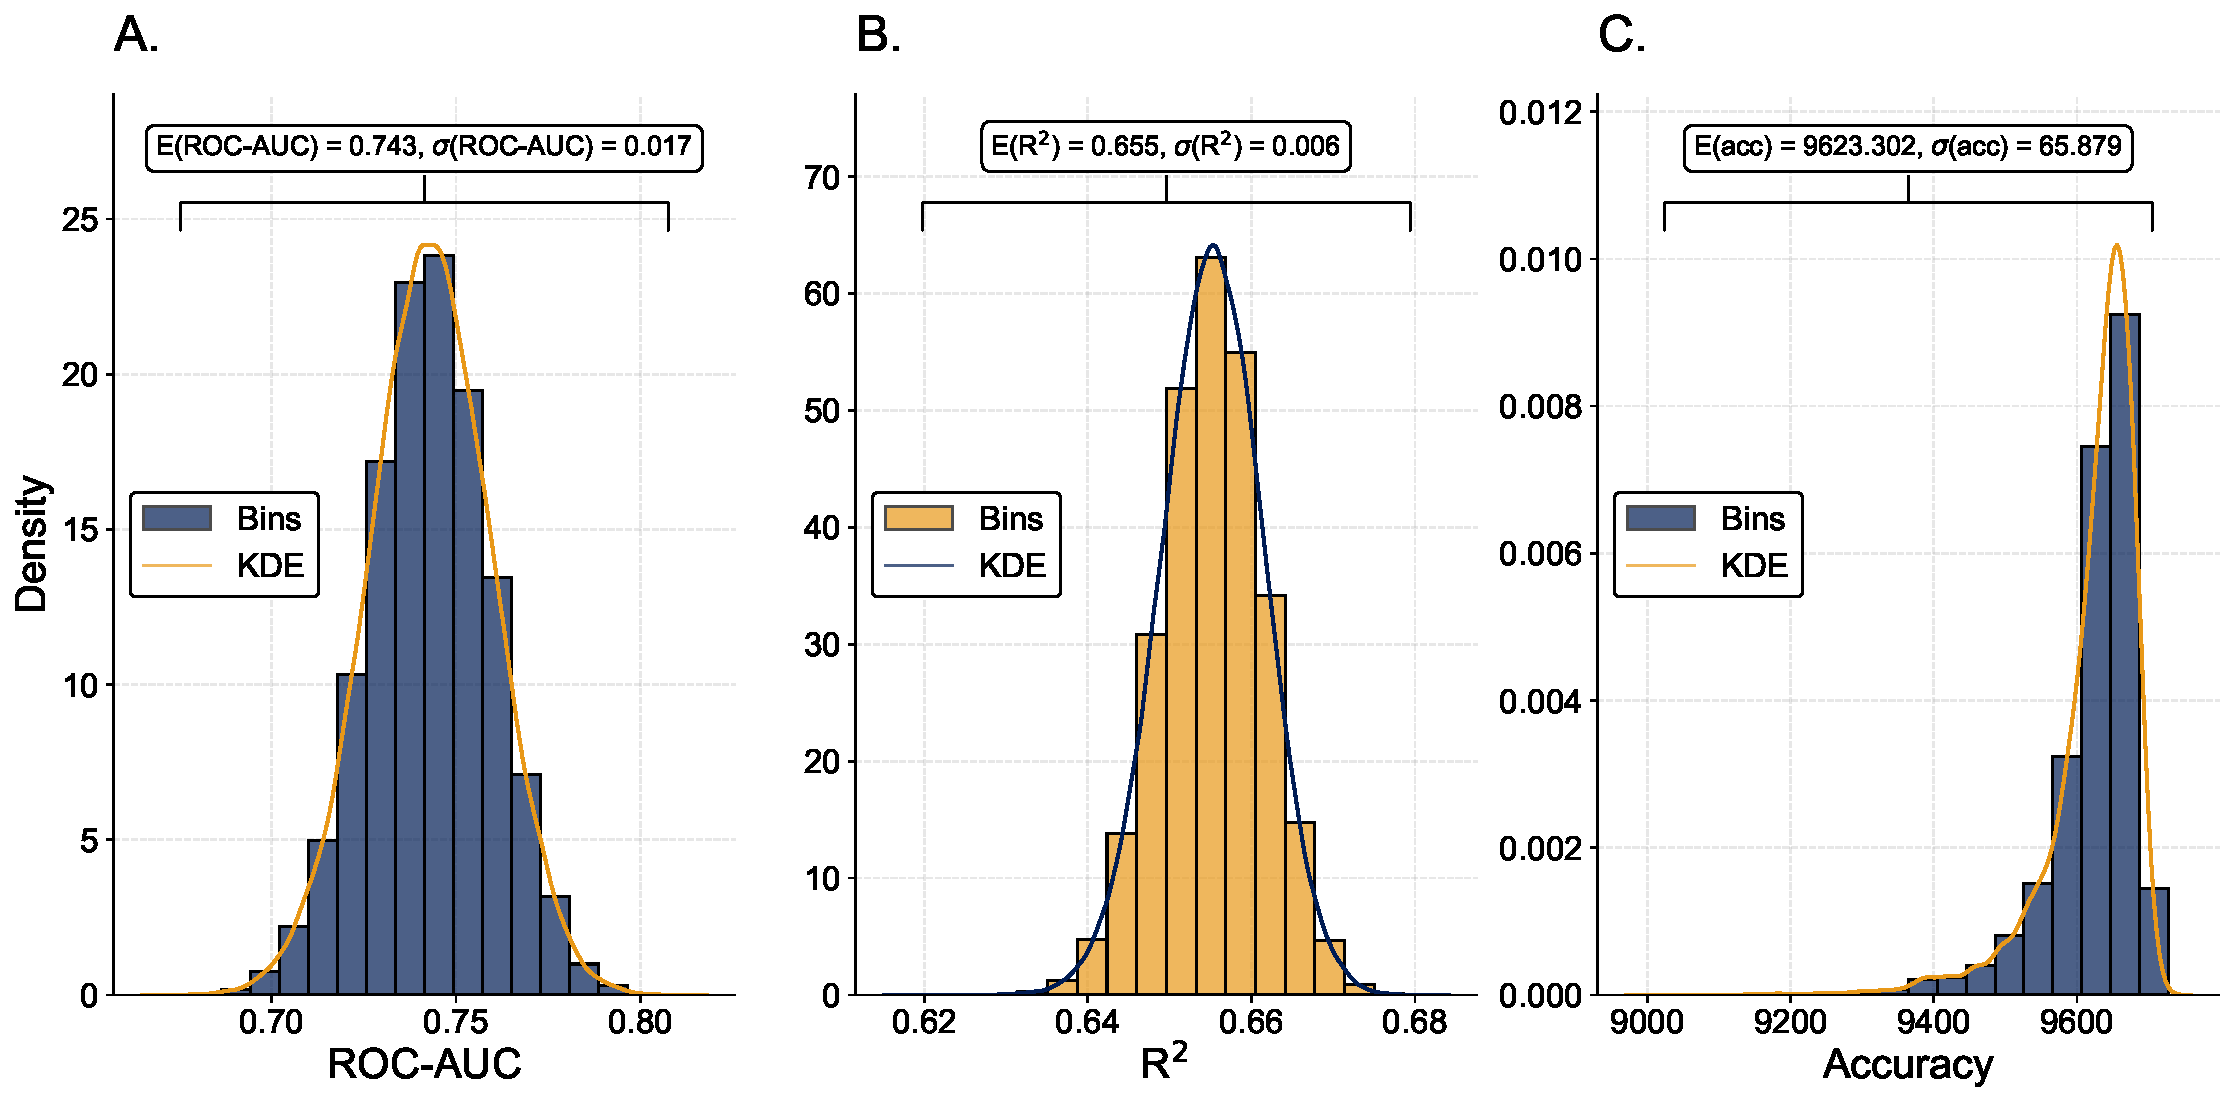
\includegraphics[width=\textwidth]{figures/prediction_seeds.pdf}
		\end{figure}
	\end{center}
\end{frame}

\section{Simple Simulations}
\begin{frame}
	\begin{center}
		\begin{figure}
			\includegraphics[width=1\textwidth]{figures/four_simple_examples.pdf}
		\end{figure}
	\end{center}
\end{frame}


\section{More Complex Replications}

\begin{frame}
\frametitle{More Complex Replications}
\begin{itemize}
    \item Lets move into more complex and direct replications.\vspace{.075in}
    \begin{itemize}
        \item[-] Major focus on the quantitative/computational social sciences.
            \begin{columns}
                \hspace{6em} % This adds the indentation
                \begin{column}{0.44\textwidth}
                    \begin{itemize}
                       \item Machine/Deep Learning
                       \item Sociology
                       \item Digital Humanities
                    \end{itemize}
                \end{column}       
                \begin{column}{0.56\textwidth}
                    \begin{itemize}
                        \item Econometrics
                        \item Time Series Analysis
                        \item Urban Segregation
                    \end{itemize}
                \end{column}
             \end{columns} 
             \vspace{.15in}
        \end{itemize}
    \item Both recent and classical papers.\vspace{.075in}
    \begin{itemize}
    \item[-] For each example, we'll give intuition as to what's going on.\vspace{.075in}
    \end{itemize}
    \item In total, this project replicates about 15 different papers.
\end{itemize}
\end{frame}

\begin{frame}
\begin{center}
\begin{figure}
	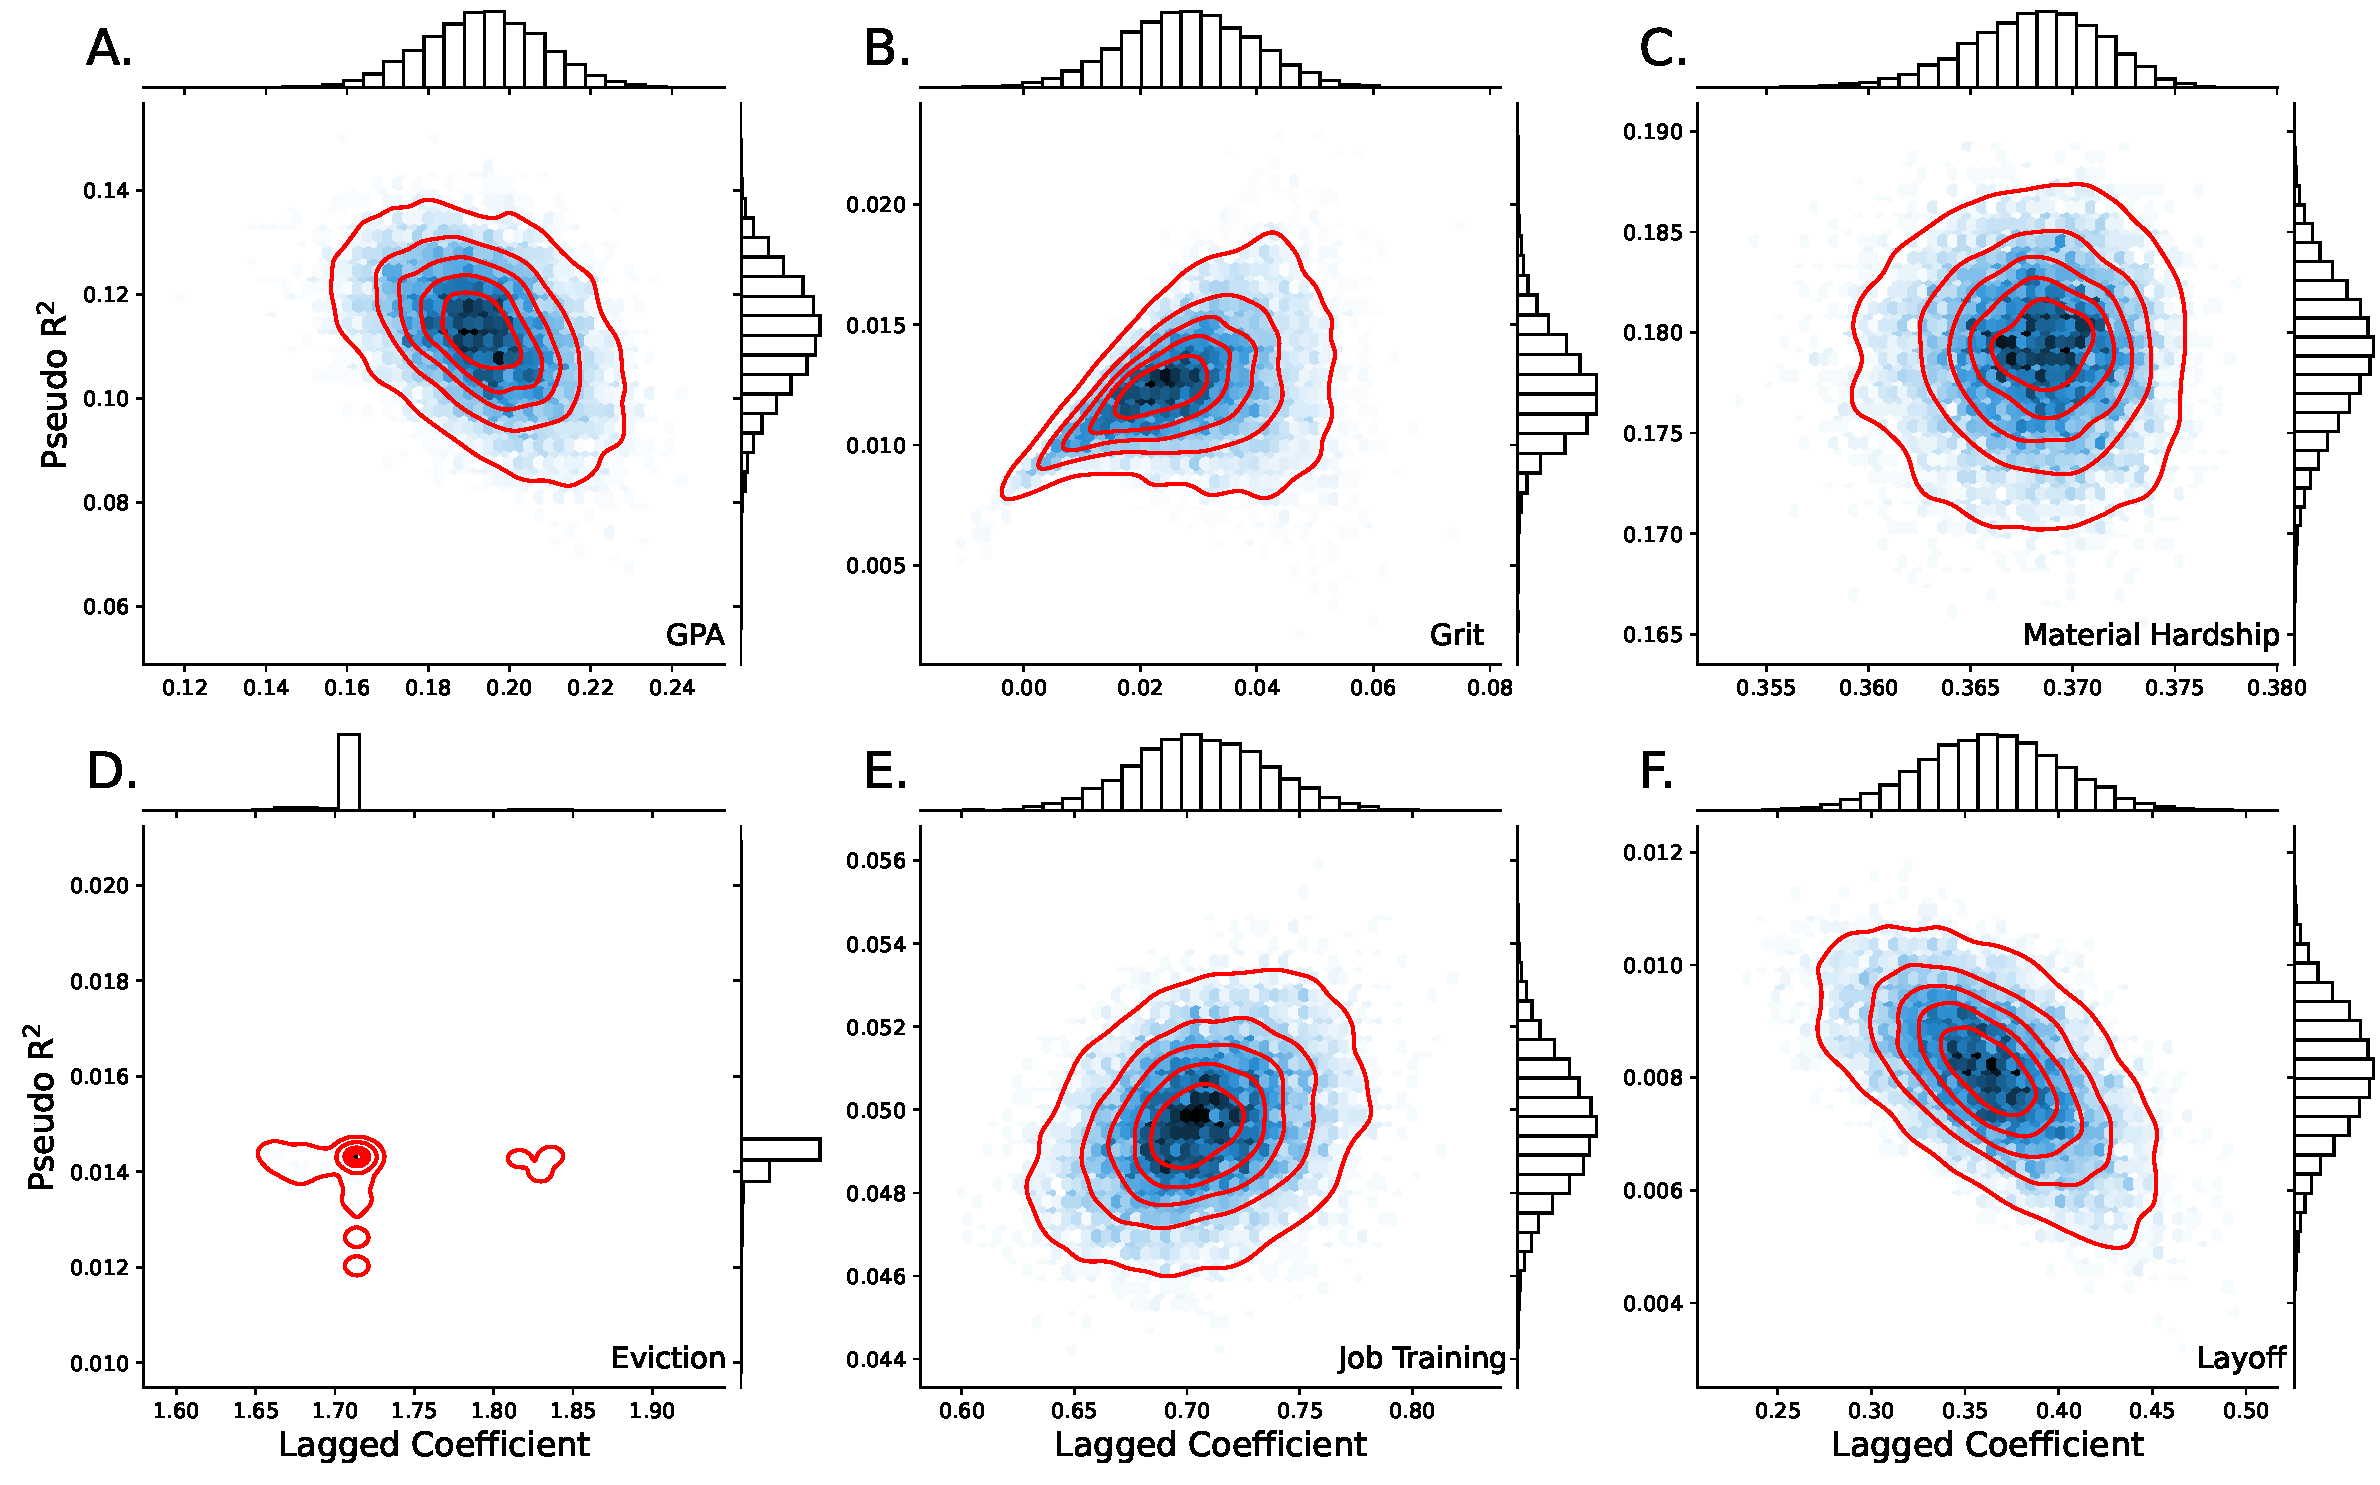
\includegraphics[width=0.95\textwidth]{figures/ffc_seeds.pdf}
\end{figure}
\end{center}
\end{frame}


\begin{frame}
\frametitle{What's going on here?}
\begin{itemize}
    \item Amelia fills in missing data by drawing values from distributions.\vspace{.1in}
    \item These distributions are based on observed data patterns.\vspace{.1in}
    \item The imputed values reflect the uncertainty in the missing data.\vspace{.1in}
	\item This is a form of \emph{Multiple Imputation}.\vspace{.1in}
	\item This results in entirely different models being built.\vspace{.1in}
	\item This has implications for both inference and prediction.\vspace{.1in}
\end{itemize}
\end{frame}


\begin{frame}
\begin{center}
\begin{figure}
	\includegraphics[width=0.95\textwidth]{figures/topic_modelling_seeds_histplot.pdf}
\end{figure}
\end{center}
\end{frame}

\begin{frame}
\frametitle{What's going on here?}
	\begin{itemize}
	    \item BERTopic has many process: one particularly volatile to seeds.\vspace{.1in}
		\item It commonly involves \emph{dimension reduction} via UMAP.\vspace{.1in}
		\begin{itemize}
		    \item \textbf{UMAP}: causes different low-dimensional embeddings.\vspace{.1in}
		\end{itemize}
		\item Note: CUML implementation of UMAP gives variable outputs for spectral initialisation \textit{even when setting the seed}.\vspace{.1in}
		\item If using HDBScan for clustering, no seed variability.\vspace{.1in}
		\item In general here, the seed variance looks \textbf{enormous}.
	\end{itemize}
\end{frame}

\begin{frame}
\begin{center}
\begin{figure}
	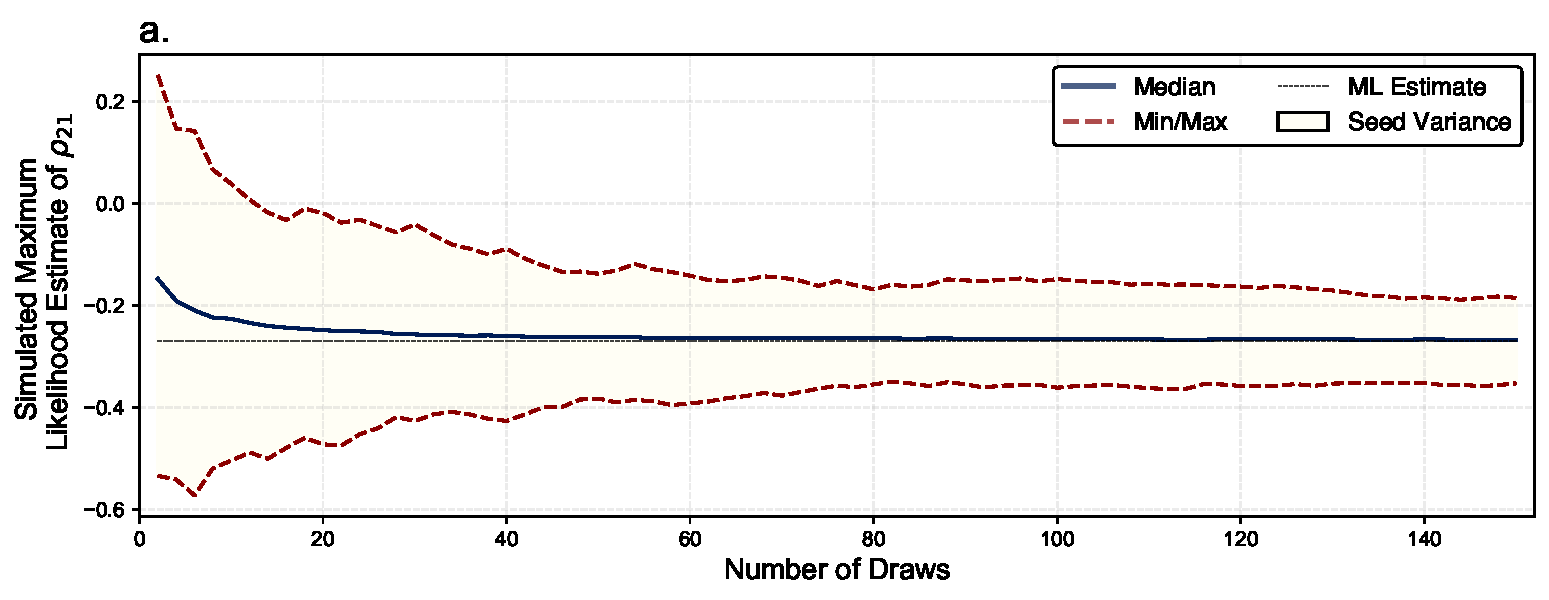
\includegraphics[width=0.95\textwidth]{./figures/mvprobit.pdf}
\end{figure}
\end{center}
\end{frame}

\begin{frame}
\frametitle{What's going on here?}


\begin{itemize}
\item The \texttt{mvprobit} estimator requires evaluating $M$ integrals jointly.\vspace{.1in}
\item This can be rewritten into a multivariate normal distributions.\vspace{.1in}
\begin{itemize}
\item Then, a sequence of normal distributions with certain properties.\vspace{.1in}
\end{itemize}
\item \texttt{mvprobit} samples from this to get at the underlying likelihood.\vspace{.1in}
\item Rewrite each individual normal to its CDF, which allows you to sample by just entering a uniform value between [0,1].\vspace{.1in}
\begin{itemize}
\item This random value is seed-dependent.\vspace{.1in}
\end{itemize}
\item Where CDF is steep on a small interval, seeds matter a lot.
\end{itemize}
%Imagine a very narrow CDF that goes from 0 to 1 on the interval [0.52, 0.53] then you need to get very lucky with a set of 10 uniforms to correctly capture the PDF by sampling from the CDF. This is where the variability comes from..

\end{frame}

\begin{frame}
	\begin{center}
		\begin{figure}
			\includegraphics[width=1\textwidth]{figures/schelling.pdf}
		\end{figure}
	\end{center}
\end{frame}



\begin{frame}
\frametitle{What's going on here?}
	\begin{itemize}
	    \item There are \textit{multiple} (!) sources of PRNG in the Schelling Model:\vspace{.1in}
		\begin{enumerate}
			\item The initialisation of the agents on the grid.\vspace{.1in}
			\item The shuffling of unhappy agents and empty cells.\vspace{.1in}
		\end{enumerate}
	\item Agents might start more/less segregated from the beginning.\vspace{.1in}
\begin{itemize}
\item This affects the speed of total segregation over time.\vspace{.1in}
\end{itemize}
	    \item Even if the model reaches similar segregation, configuration of agents and trajectories will differ.\vspace{.1in}
	\item As shown in the previous slide, parameterisation matters (a lot).\vspace{.1in}
	\end{itemize}
\end{frame}


\begin{frame}
	\begin{center}
		\begin{figure}
			\includegraphics[width=1\textwidth]{figures/four_rws.pdf}
		\end{figure}
	\end{center}
\end{frame}

\begin{frame}
\frametitle{What's going on here?}
	\begin{itemize}
	    \item Seeds modify sequences of PRNG draws, affecting $y_t$.\vspace{.065in}
	    \item Moments of previous changes ($\mu$, $\sigma/2$) control magnitude.\vspace{.065in}
	    \item Draws of $\mathcal{N}(\mu, \sigma/2)$ impact asset price trajectory.\vspace{.065in}
	    \item The seed affects long-term trends by influencing both direction and size of early random steps.\vspace{.065in}
	\end{itemize}
This can be formally written as:
\begin{equation}
y_t = y_{t-1} + \epsilon_t \quad \text{where} \quad \epsilon_t \sim \mathcal{N}(\mu, \sigma/2)
\end{equation}

\begin{itemize}
	\item Previously thought that nothing outperforms RW for ForEx.\vspace{.065in}
	\item RWs commonly used as a benchmark for structural models.
\end{itemize}
\end{frame}

%\section{Collisions}
%\begin{frame}
%\begin{small}
%\frametitle{To make things more complicated...}
%\begin{itemize}
%\item Hofert (2020): in \textit{some} scenarios, \textbf{collisions} exist.\\ \vspace{.01in}
%\item Collisions: generation of duplicates b/c of insufficient complexity.\\ \vspace{.01in}
%\item An author of a leading LCDS publication recently  stated to me:\\ \vspace{.01in}
%\end{itemize}
%\begin{quote}
%\begin{small}
%\begin{center}
%``We wanted to run it [the model] with a 100k seeds, but in reality, it was only 99,905 or something, %because we were seeing that our results weren't unique when they should have been.''
%\end{center}
%\end{small}
%\end{quote}
%\begin{itemize}
%\item This \textit{only} occurs in 32-bit Mersenne Twister implementations.\\ \vspace{.01in}
%\begin{itemize}
%\item With 32-bit MT: E(collisions) is 116.\\ \vspace{.01in}
%\item With 64-bit MT: E(collisions is 2.71e-08.\\ \vspace{.01in}
%\end{itemize}
%\item The default implementation of MT in \texttt{R} is 32-bit$\hdots$.
%\end{itemize}
%\end{small}
%\end{frame}

%\begin{frame}
%\begin{center}
%\begin{figure}
%\includegraphics[width=.925\linewidth]{../../figures//collisions} \\ \vspace{.025in}
%\end{figure}
%\end{center}
%\end{frame}


\section{Concluding Thoughts}
\begin{frame}
\frametitle{Concluding Thoughts (Part One)}
\begin{itemize}
\item Matt Salganik commented: `That sounds great, but expensive!'\\ \vspace{.05in}
\begin{itemize}
\item Expense no-longer prohibitive: everything here ran locally.\\ \vspace{.035in}
\item We live in an age of vast computational resources.\pause \\ \vspace{.06in}
\end{itemize}
\item What are our suggestions?\pause \\ \vspace{.06in}
\begin{itemize}
\item \textbf{Researchers:} Visualize your seed variability where affordable!\\ \vspace{.035in}
\begin{itemize}
	\item There are times when you can eliminate/reduce seed variability.\\ \vspace{.04in}
	\item Pedagogically, lets teach students to parralelize code effectively.\\ \vspace{.04in} \pause
\end{itemize}
\item \textbf{Reviewers:} Question papers you read -- is there stochasticity?\pause \\ \vspace{.04in}
\begin{itemize}
	\item Even well established results are susceptible.\\ \vspace{.04in} \pause
\end{itemize}
\item \textbf{Editors:} Ubiquitous mandate for responsible use of PRNGs!
\end{itemize}
\end{itemize}
\end{frame}











\begin{frame}[fragile]
\begin{center}
\begin{scriptsize}
\begin{minipage}{.9\linewidth}
\begin{myenv}{simple\_seed\_algorithm.py}
\begin{minted}{Python}

import numpy as np # for randomisation
import matplotlib.pyplot as plt # for plotting

def analytical_function(input, seed):
	''' Simple analytical function: can be anything'''
	np.random.seed(seed)
	return input*np.random.normal()

results = [] # store results
inputs = 42 # dataset, figure path, etc.

for seed in range(0, 100000): # simple loop; can be distributed
	results.append(analytical_function(inputs, seed))

plt.hist(results) # plot results
\end{minted}
\end{myenv}
\end{minipage}
\end{scriptsize}
\end{center}
\end{frame}


\begin{frame}[fragile]
\begin{center}
\begin{scriptsize}
\begin{minipage}{.9\linewidth}
\begin{myenv}{better\_seed\_algorithm.py}
\begin{minted}{Python}

import numpy as np # for randomisation
import matplotlib.pyplot as plt # for plotting

def analytical_function(input, seed):
	''' Simple analytical function: can be anything'''
	np.random.seed(seed)
	return input*np.random.normal()

results = [] # store results
inputs = 42 # dataset, figure path, etc.

# Instead, use list of predefined, complex 'secret' seeds we provide
with open(os.path.join( '..', 'assets', 'seed_list.txt')) as f:
    seed_list = [int(line.rstrip('\n')) for line in f]

for seed in seed_list: # simple loop; can be distributed
	results.append(analytical_function(inputs, seed))

plt.hist(results) # plot results
\end{minted}
\end{myenv}
\end{minipage}
\end{scriptsize}
\end{center}
\end{frame}











\begin{frame}
\frametitle{Concluding Thoughts (Part Two)}
\begin{itemize}
\item Ideally, we want to move towards \emph{distributional} reproducibility.\\ \vspace{.1in}
\item Moving foward, PRGNs \emph{shouldn't} exist (QRNGs the norm).\\ \vspace{.1in}
\item Does anyone have ideas for other types of seed variability?\\ \vspace{.1in}
\item Can this be corrective? Index historical seed variability?\\ \vspace{.1in}
\item Prospectively: we make available a list of seeds (replication materials), encouraging their use as a pre-specified set.\\ \vspace{.1in}
\item \textbf{TLDR}: when variation can't be eliminated, should be visualised.
\end{itemize}
\end{frame}

\begin{frame}
\frametitle{Thanks to my Coauthors!}
\begin{figure}[h]
    \centering
    \begin{subfigure}[b]{0.45\textwidth}
        \centering
        \includegraphics[width=0.75\textwidth]{figures/mark-modified.png} % Replace with your image file
        \caption*{\quad \quad \quad \quad \quad Mark Verhagen}
        \label{fig:image1}
    \end{subfigure}
    \hfill \vspace{.15in}
    \begin{subfigure}[b]{0.45\textwidth}
        \centering
        \includegraphics[width=0.75\textwidth]{figures/jiani-modified.png} % Replace with your image file
        \caption*{\quad \quad \quad \quad \quad \quad Jiani Yan}
        \label{fig:image2}
    \end{subfigure}
%    \caption{Overall caption for the two images}
    \label{fig:two_images}
\end{figure}\pause
\begin{center}
And \emph{thanks to you for your attention and attedance!}
\end{center}
\end{frame}

\end{document}
